\documentclass[12pt,a4paper,oneside,titlepage] {article}

\usepackage[T2A]{fontenc}
\usepackage[utf8]{inputenc}
\usepackage[russian]{babel}
\usepackage{hyperref}
\usepackage{multicol}
\usepackage{listings}
\usepackage{geometry}
\usepackage{minted}

\usepackage{graphicx}
\graphicspath{ {./images/} }
\usepackage{wrapfig}

\begin{document}

% НАЧАЛО ТИТУЛЬНОГО ЛИСТА
\begin{center}
  \hfill
  \break
  \textbf{
    \footnotesize{Министерство науки и высшего образования Российской Федерации}\\
    \hfill \break
    \footnotesize{Федеральное государственное бюджетное образовательное учреждение высшего образования}\\
    \small{«МОСКОВСКИЙ ГОСУДАРСТВЕННЫЙ ТЕХНИЧЕСКИЙ УНИВЕРСИТЕТ имени Н.Э.БАУМАНА\\(национальный исследовательский университет)»}}\\
    \footnotesize{(МГТУ им. Н.Э. Баумана)}\\
    
\includegraphics[width=25mm,scale=0.25]{emblem}
\end{center}
\hfill
\break
\normalsize{Факультет: Информатика и системы управления}\\
\hfill \break
\normalsize{Кафедра: Теоретическая информатика и компьютерные технологии}\\
\hfill\break
\begin{center}
  \textbf{\large{Лабораторная работа №{{.labNumber}}}}\\
  \large{{{.labName}}}\\
  \textbf{\large{Вариант {{.labVariant}}}}\\
\end{center}
\hfill \break
\hfill \break
\hfill \break
\hfill \break
\hfill \break
\hfill \break
\hfill \break
\hfill \break
\begin{flushright}
  \normalsize{
    Выполнил\\
    студент группы ИУ9-31Б\\
    Лисов Алексей
  }
\end{flushright}

\hfill \break
\begin{center} Москва, 2023 \end{center}
\thispagestyle{empty} % выключаем отображение номера для этой страницы
% КОНЕЦ ТИТУЛЬНОГО ЛИСТА

\section{Условие}
{{.statement}} Условие задачи, исходный код и пример работы программы необходимо предоставить в формате \LaTeX.

\section{Код решения}

{{.code}}


\begin{figure}[H]
	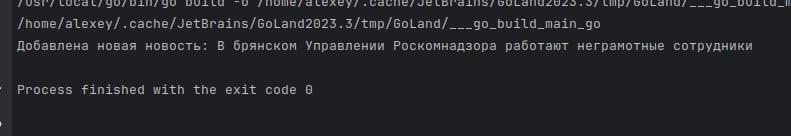
\includegraphics[width=300px,scale=0.25]{blah.jpg}
    \centering
    \caption{Код}
    \label{fig:my_label}
\end{figure}

\begin{figure}[H]
	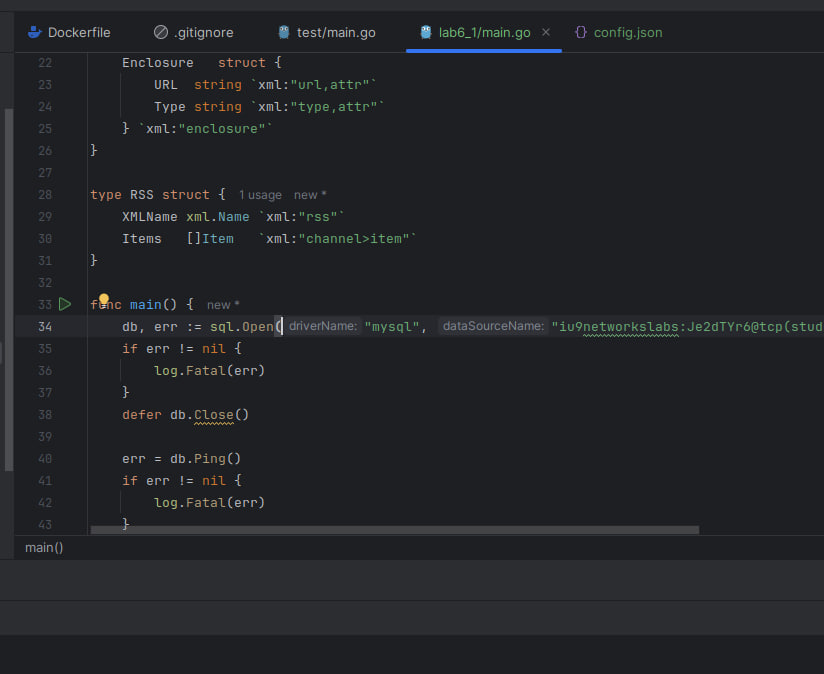
\includegraphics[width=300px,scale=0.25]{blahblah.jpg}
    \centering
    \caption{Код}
    \label{fig:my_label}
\end{figure}

\end{document}
